\section{Statistics}
We maintain a Germinate statistics page on our server. It shows an overview of all Germinate instances that we currently maintain. It's available at:
\begin{center}
	\url{http://ics.hutton.ac.uk/germinate/germinate-statistics}
\end{center}
\noindent
Figure \ref{fig:statistics-overview-table} shows one of the visualizations we provide. We're planning to add more visualizations in the future. Now you might think: "What does that have to do with me?".

The answer is simple: We can add your instance of Germinate to our statistics website. That way, people browsing our website may stumble across your site which can broaden your potential target audience. In addition, access to statistical data from more Germinate instances allows us to improve Germinate and the statistics page. So it's basically a win-win situation.\\
\\
If you are interested and want us to add your Germinate instance to our statistics page, or if you have any questions, drop us an email: \url{germinate@hutton.ac.uk}.\\
\\
Just in case you are wondering what kind of data we would collect from your Germinate instance, let me go into detail here: When you start Germinate on your server, it creates a couple of views. These views contain the aggregated data. You can examine these views with your favourite MySQL tool. Let me stress, that these views by themselves are not visible to anyone but you, so there is nothing to worry about.

For us to be able to use these views, you would need to create a new database user that has \texttt{select} and \texttt{show view} privileges on the views. Please note, that this user will not have select access to the database tables, so your actual data is safe. We would then store the user credentials in our database and run a query against your views once a day. Consequently, the data we show on our statistics page is always up to date.

\begin{figure}
	\centering
	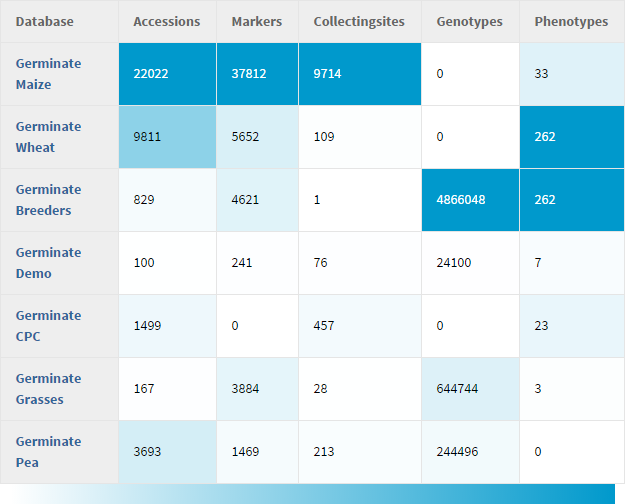
\includegraphics[scale=0.6]{img/statistics/overview-table.png}
	\caption{Statistics overview table}
	\label{fig:statistics-overview-table}
\end{figure}